\chapter{WAN Architectures}\label{wan-architectures}

\section{Introduction to WANS}\label{introduction-to-wans}

\begin{itemize}
\tightlist
\item
  WAN stands for WIDE AREA NETWORK
\item
  A WAN is a NETWORK that extends over a large geographic area
\item
  WANs are used to connect geographically separate LANs
\item
  Although the Internet can be considered a WAN, the term ``WAN'' is
  typically used to refer to an enterprise's private connections that
  connect their offices, data centers, and other sites together
\item
  Over public/shared networks like the Internet, VPNs (Virtual Private
  Networks) can be used to create private WAN connections
\item
  There have been many different WAN technologies over the years.
  Depending on the location, some will be available and some will not be
\item
  Technologies which are considered ``legacy'' (old) in one country,
  might still be used in other countries
\end{itemize}

\section{WAN over Dedicated Connection (Leased
Line)}\label{wan-over-dedicated-connection-leased-line}

HUB-and-SPOKE topology

\begin{figure}
\centering
\pandocbounded{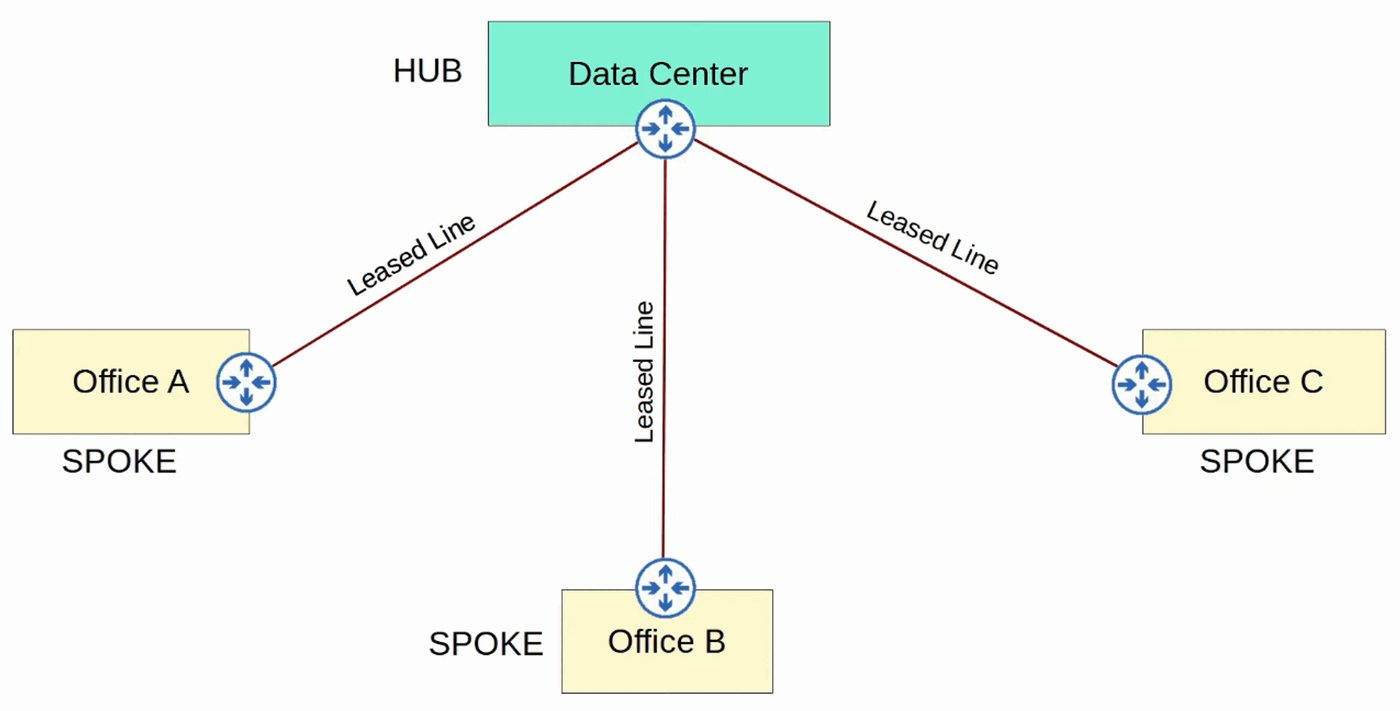
\includegraphics[keepaspectratio,alt={image}]{images/54-wan-architectures/img-001.png}}
\end{figure}

\begin{figure}
\centering
\pandocbounded{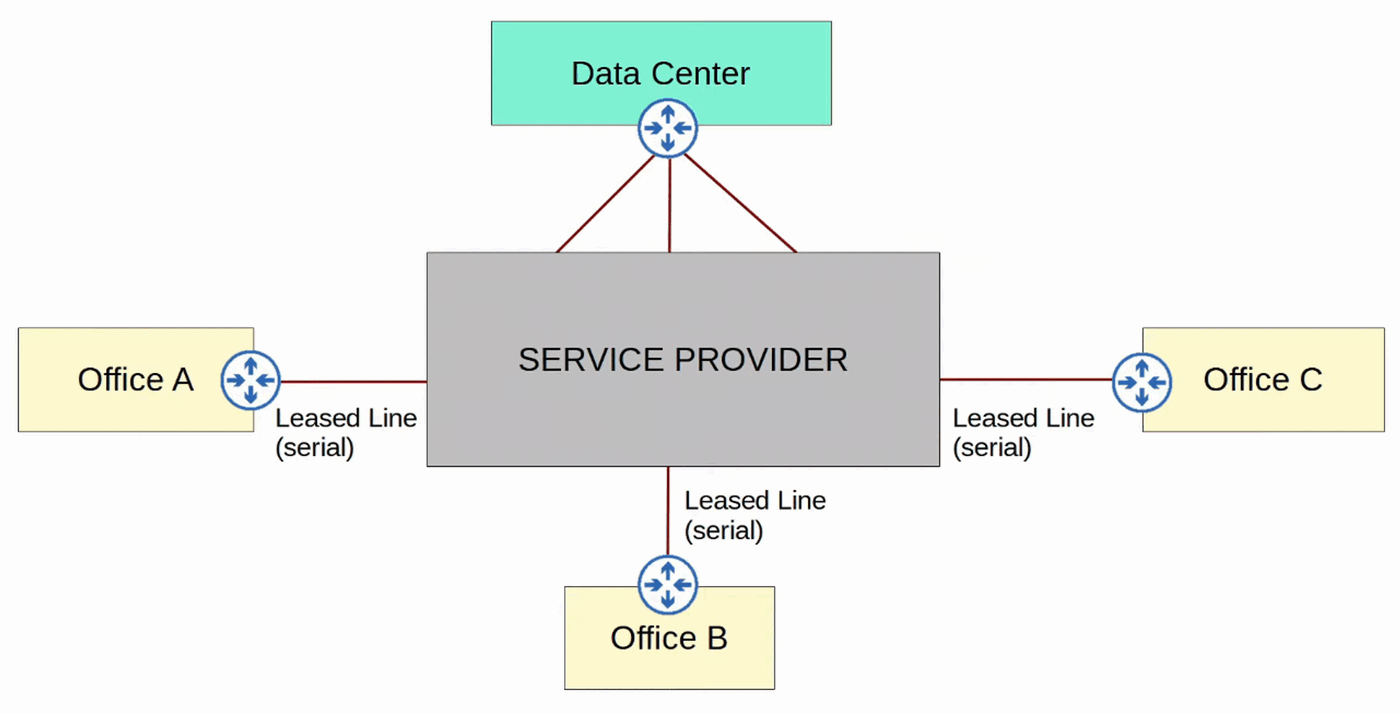
\includegraphics[keepaspectratio,alt={image}]{images/54-wan-architectures/img-002.png}}
\end{figure}

\section{WAN Connection Via Ethernet
(Fiber)}\label{wan-connection-via-ethernet-fiber}

\begin{figure}
\centering
\pandocbounded{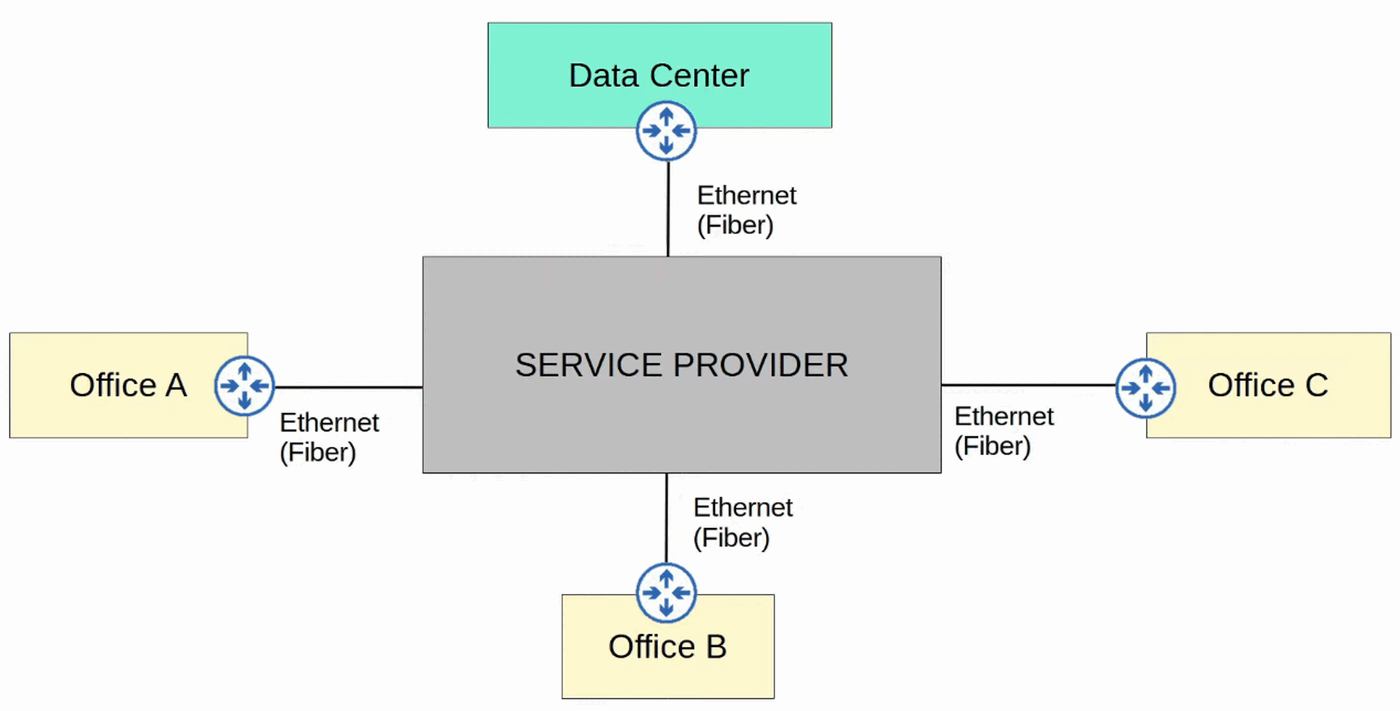
\includegraphics[keepaspectratio,alt={image}]{images/54-wan-architectures/img-003.png}}
\end{figure}

\section{WAN over Shared Infrastructure (Internet
VPN)}\label{wan-over-shared-infrastructure-internet-vpn}

\begin{figure}
\centering
\pandocbounded{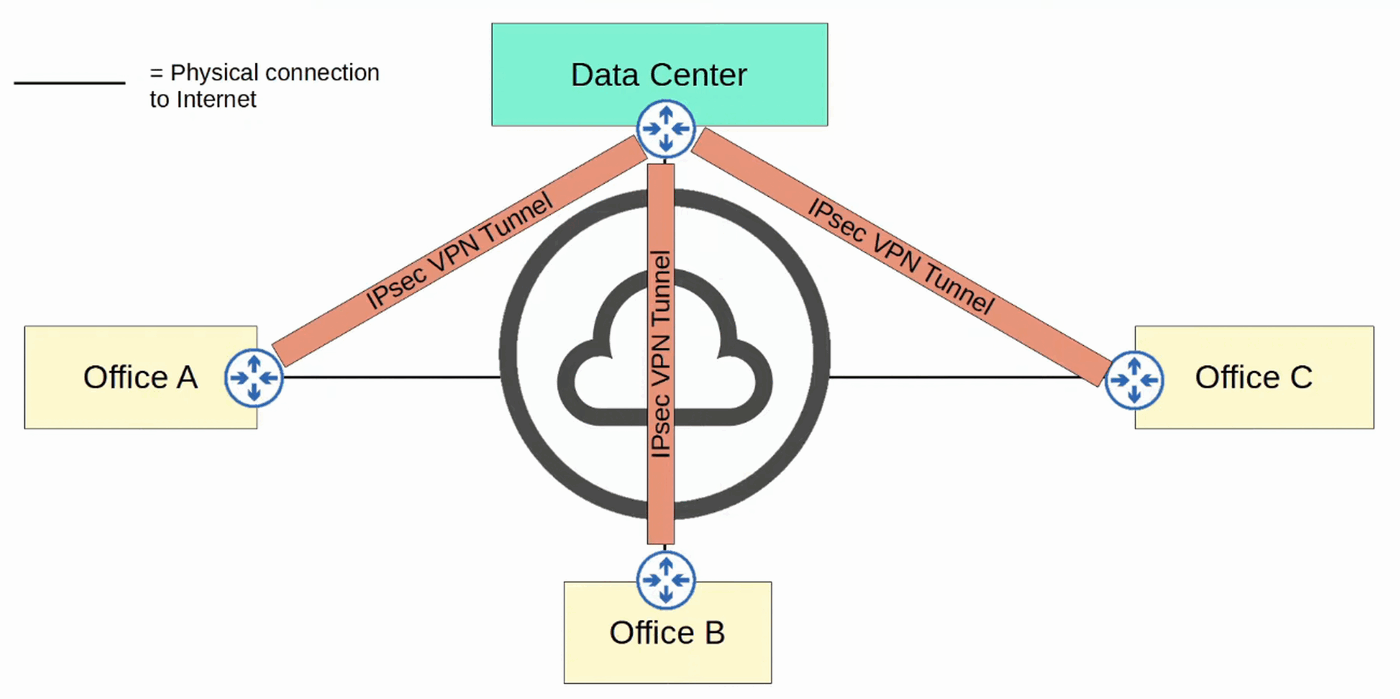
\includegraphics[keepaspectratio,alt={image}]{images/54-wan-architectures/img-004.png}}
\end{figure}

\section{Leased Lines}\label{leased-lines}

\begin{itemize}
\tightlist
\item
  A LEASED LINE is a dedicated physical link, typically connecting two
  sites
\item
  LEASED LINES use serial connections (PPP or HDLC encapsulation)
\item
  There are various standards that provide different speeds and
  different standards are available in different countries.
\item
  Due to the HIGHER cost, HIGHER installation lead time, and SLOWER
  speeds of LEASED LINES, Ethernet WAN technologies are becoming MORE
  popular
\end{itemize}

\begin{figure}
\centering
\pandocbounded{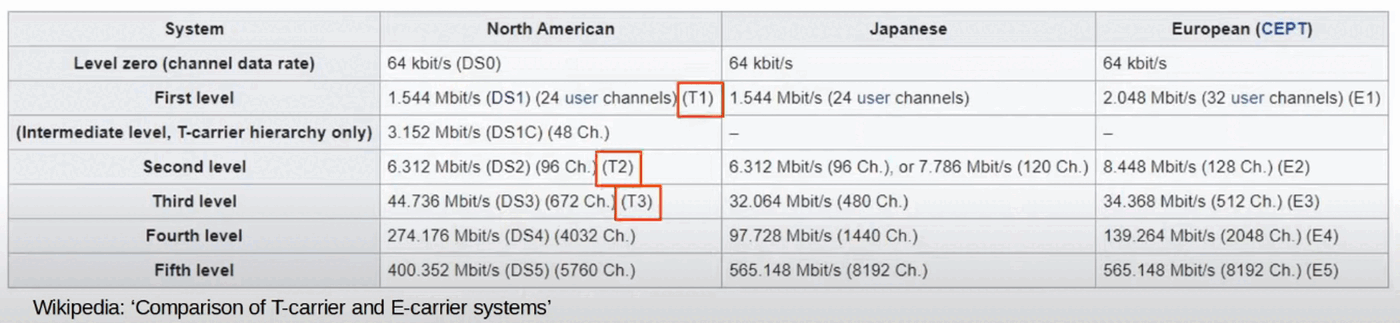
\includegraphics[keepaspectratio,alt={image}]{images/54-wan-architectures/img-005.png}}
\end{figure}

MPLS VPNs

\begin{itemize}
\tightlist
\item
  MPLS stands for ``Multi Protocol Label Switching''
\item
  Similar to the Internet, service providers' MPLS NETWORKS are shared
  infrastructure because many customer enterprises connect to and share
  the same infrastructure to make WAN connections
\item
  However, the ``label switching'' in the name of MPLS allows VPNs to be
  created over the MPLS infrastructure through the use of LABELS
\item
  IMPORTANT terms:

  \begin{itemize}
  \tightlist
  \item
    CE ROUTER = Customer Edge ROUTER
  \item
    PE ROUTER = Provider Edge ROUTER
  \item
    P ROUTER = Provider Core ROUTER
  \end{itemize}
\end{itemize}

\begin{figure}
\centering
\pandocbounded{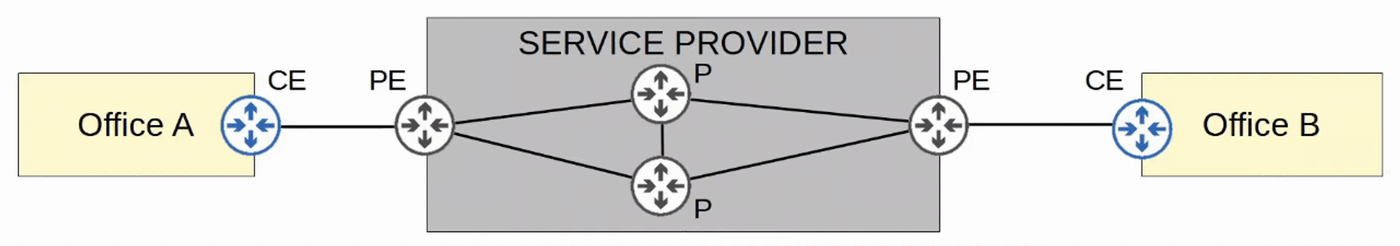
\includegraphics[keepaspectratio,alt={image}]{images/54-wan-architectures/img-006.png}}
\end{figure}

\begin{itemize}
\tightlist
\item
  When the PE ROUTERS receive FRAMES from the CE ROUTERS, they add a
  LABEL to the FRAME
\item
  These LABELS are used to make forwarding decisions within the SERVICE
  PROVIDER NETWORK - NOT the DESTINATION IP
\item
  The CE ROUTERS do NOT USE MPLS, it is only used by the PE/P ROUTERS
\item
  When using a LAYER 3 MPLS VPN, the CE and PE ROUTERS peer using OSPF,
  for example, to share ROUTING information
\end{itemize}

\section{Example}\label{example}

OFFICE A's CE will peer with one PE

OFFICE B's CE will peer with the other PE

OFFICE A's CE will learn about OFFICE B's ROUTES via this OSPF peering

OFFICE B's CE will learn about OFFICE A's ROUTES as well

\begin{figure}
\centering
\pandocbounded{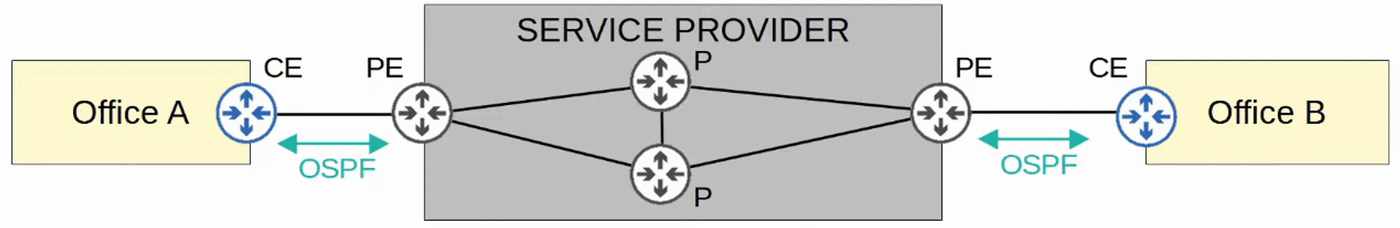
\includegraphics[keepaspectratio,alt={image}]{images/54-wan-architectures/img-007.png}}
\end{figure}

\begin{itemize}
\tightlist
\item
  When using a LAYER 2 MPLS VPN, the CE and PE ROUTERS do NOT form
  PEERINGS
\item
  The SERVICE PROVIDER NETWORK is entirely \emph{transparent} to the CE
  ROUTERS
\item
  In effect, it is like the TWO CE ROUTERS are directly connected.

  \begin{itemize}
  \tightlist
  \item
    Their WAN INTERFACES will be in the SAME SUBNET
  \end{itemize}
\item
  If a ROUTING protocol is used, the TWO CE ROUTERS will peer directly
  with each other
\end{itemize}

CE ROUTERS connected via LAYER 2 MPLS VPN

\begin{figure}
\centering
\pandocbounded{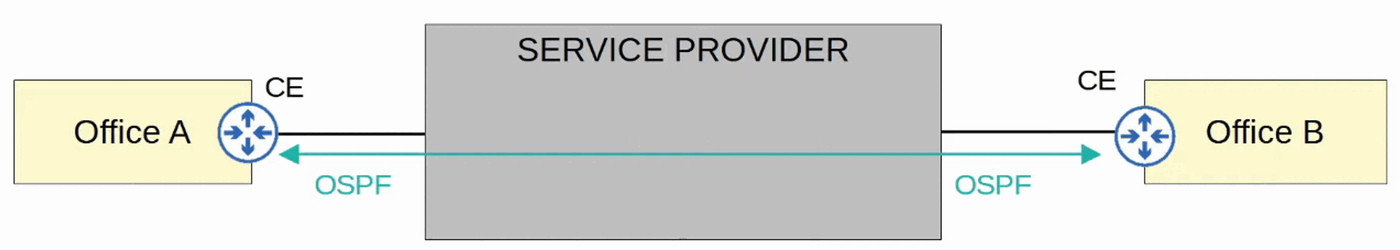
\includegraphics[keepaspectratio,alt={image}]{images/54-wan-architectures/img-008.png}}
\end{figure}

\begin{figure}
\centering
\pandocbounded{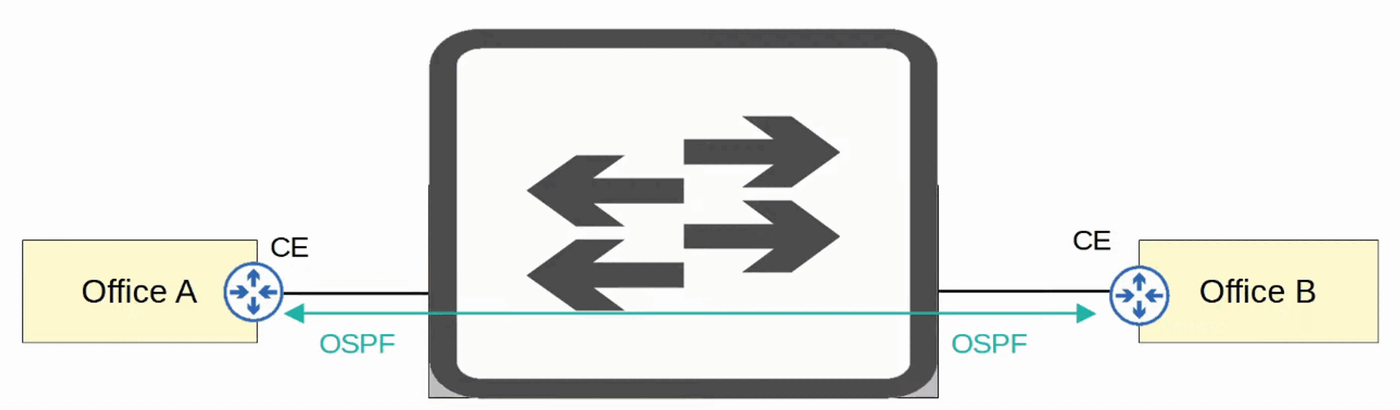
\includegraphics[keepaspectratio,alt={image}]{images/54-wan-architectures/img-009.png}}
\end{figure}

\section{Mpls}\label{mpls}

\begin{itemize}
\tightlist
\item
  Many different technologies can be used to connect to a SERVICE
  PROVIDER's MPLS NETWORK for WAN Service
\end{itemize}

\begin{figure}
\centering
\pandocbounded{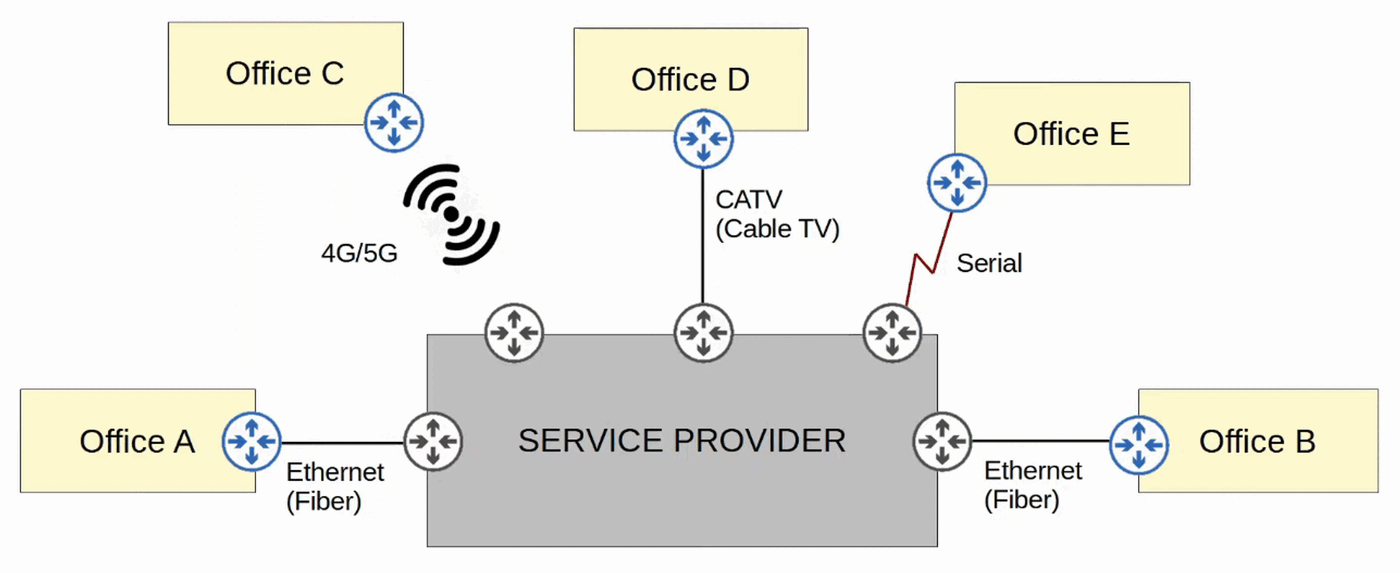
\includegraphics[keepaspectratio,alt={image}]{images/54-wan-architectures/img-010.png}}
\end{figure}

\section{Internet Connectivity}\label{internet-connectivity}

\begin{itemize}
\tightlist
\item
  There are countless ways for an enterprise to connect to the INTERNET
\item
  For example, PRIVATE WAN technologies such as LEASED LINES and MPLS
  VPNs can be used to connect to a SERVICE PROVIDER's INTERNET
  infrastructure
\item
  In addition, technologies such as CATV and DSL commonly used by
  consumers (Home Internet Access) can also be used by an enterprise
\item
  These days for both enterprise and consumer INTERNET access, FIBER
  OPTIC ETHERNET connections are growing in popularity due to high
  speeds they provide over long distances
\item
  Let's briefly look at TWO INTERNET access technologies mentioned
  above:

  \begin{itemize}
  \tightlist
  \item
    CABLE (CATV)
  \item
    DSL
  \end{itemize}
\end{itemize}

\section{Digital Subscriber Line
(DSL)}\label{digital-subscriber-line-dsl}

\begin{itemize}
\tightlist
\item
  DSL provides INTERNET connectivity to customers over phone lines and
  can share the same phone line that is already installed in most homes
\item
  A DSL MODEM (Modulator / Demodulator) is required to convert DATA into
  a format suitable to be sent over the phone lines

  \begin{itemize}
  \tightlist
  \item
    The MODEM might be a separate DEVICE or it might be incorporated in
    to a ``HOME ROUTER''
  \end{itemize}
\end{itemize}

\begin{figure}
\centering
\pandocbounded{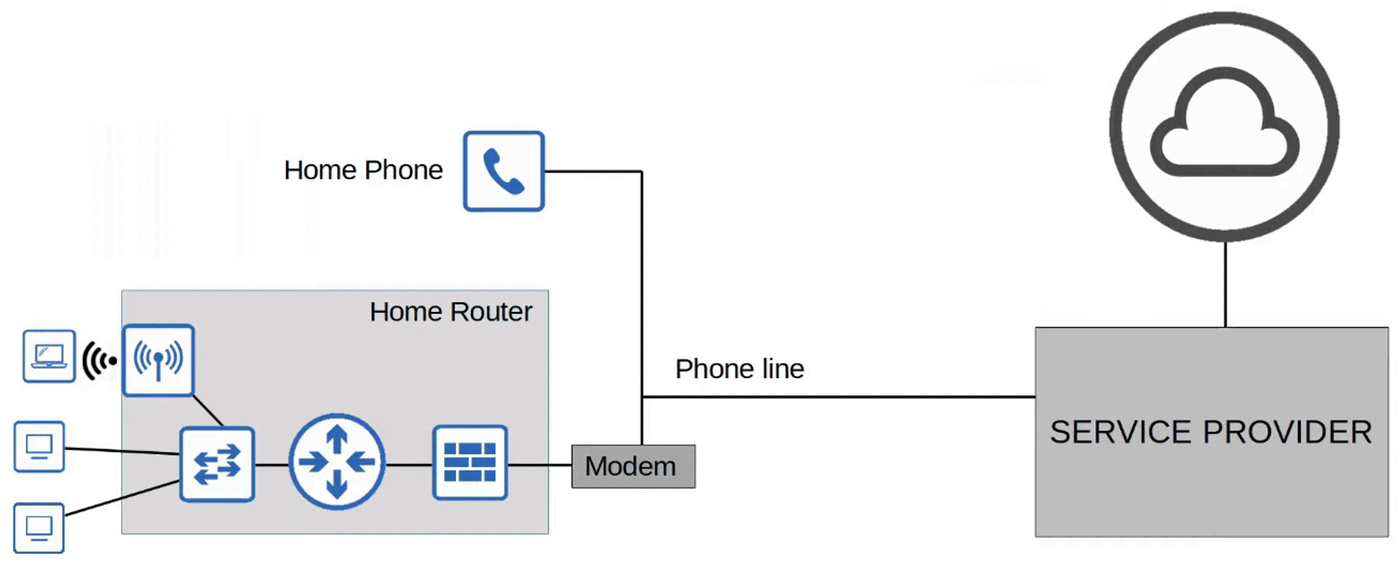
\includegraphics[keepaspectratio,alt={image}]{images/54-wan-architectures/img-011.png}}
\end{figure}

\section{Cable Internet}\label{cable-internet}

\begin{itemize}
\tightlist
\item
  CABLE INTERNET provides INTERNET ACCESS via the same CATV (Cable
  Television) lines used for TV service
\item
  Like DLS, a CABLE MODEM is required to convert DATA into a format
  suitable to be sent over the CATV CABLES.

  \begin{itemize}
  \tightlist
  \item
    Like a DSL MODEM, this can be a separate device or built into the
    HOME ROUTER
  \end{itemize}
\end{itemize}

\begin{figure}
\centering
\pandocbounded{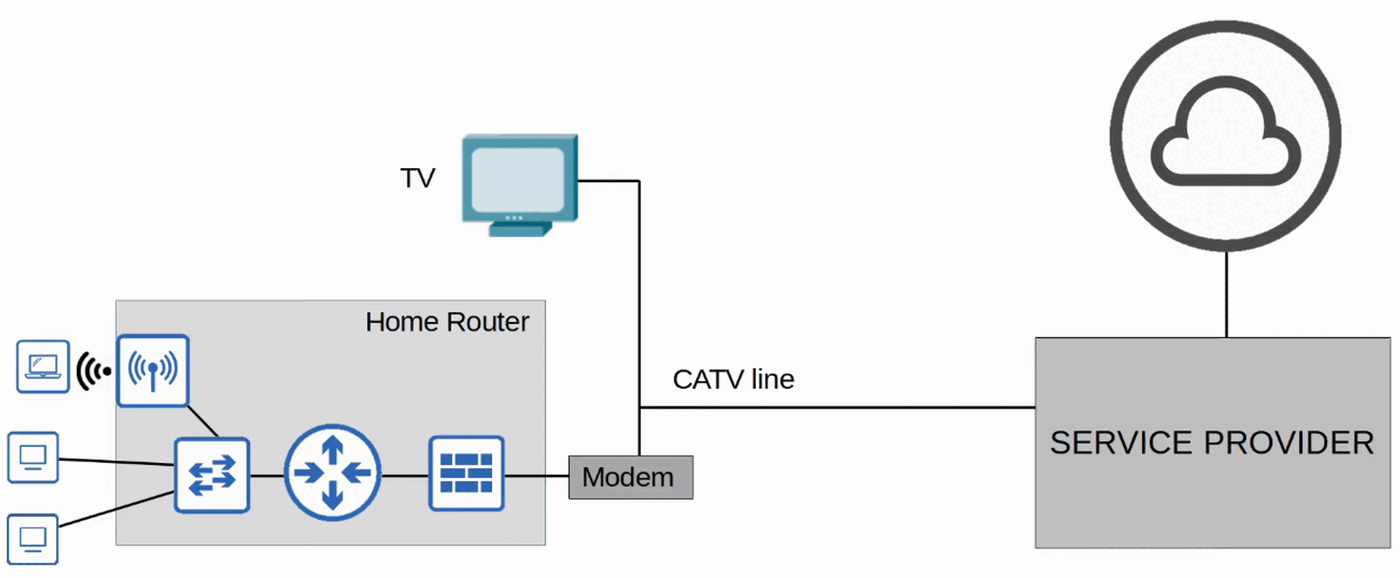
\includegraphics[keepaspectratio,alt={image}]{images/54-wan-architectures/img-012.png}}
\end{figure}

\section{Redundant Internet
Connections}\label{redundant-internet-connections}

\begin{figure}
\centering
\pandocbounded{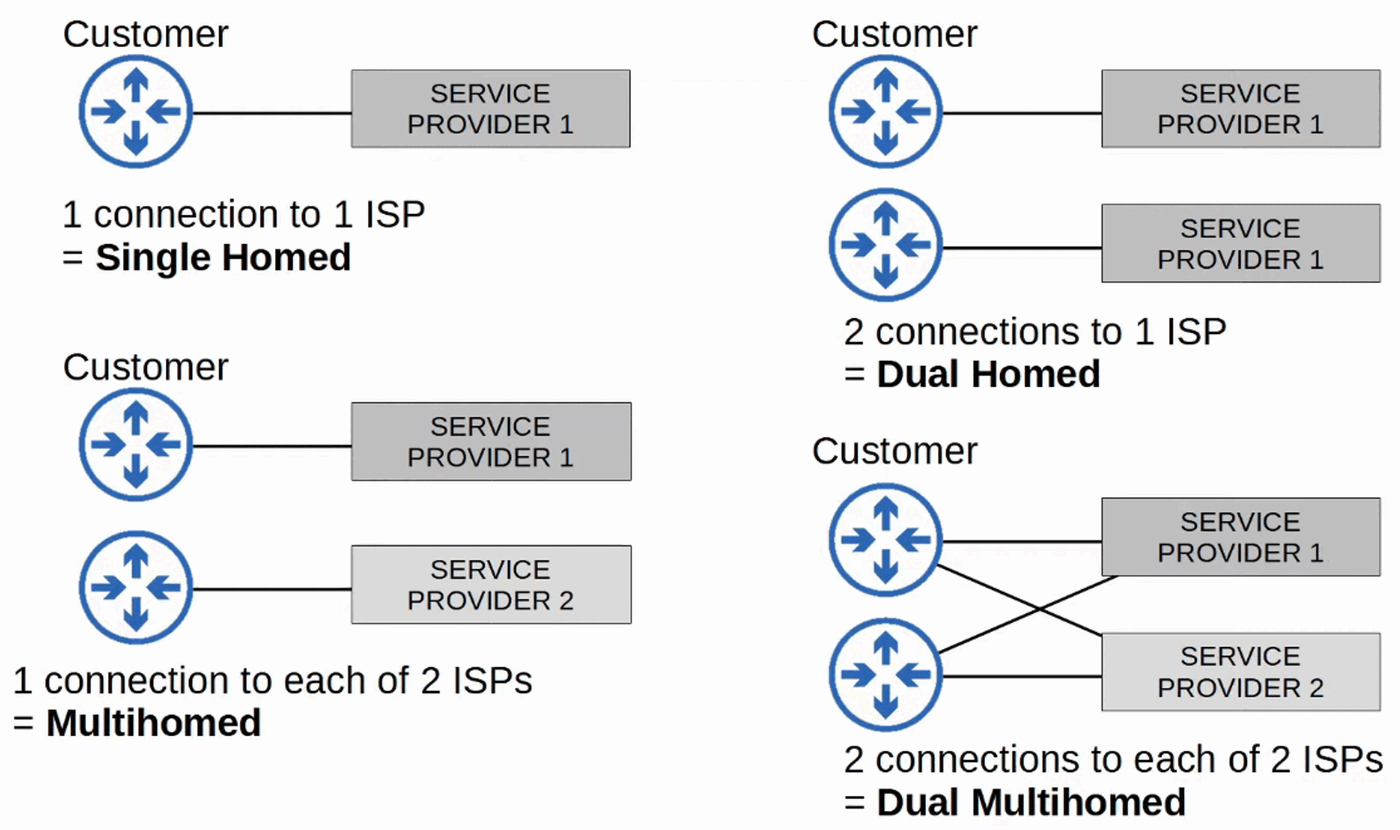
\includegraphics[keepaspectratio,alt={image}]{images/54-wan-architectures/img-013.png}}
\end{figure}

INTERNET VPNs

\begin{itemize}
\tightlist
\item
  PRIVATE WAN SERVICES such as LEASED LINES and MPLS provide security
  because each customer's TRAFFIC is separated by using dedicated
  physical connections (LEASED LINE) or by MPLS TAGS
\item
  When using the INTERNET as a WAN to connect SITES together, there is
  no built-in security by DEFAULT
\item
  To provide secure communications over the Internet, VPNs (Virtual
  Private Networks) are used
\item
  We will cover two kinds of Internet VPNs:

  \begin{itemize}
  \tightlist
  \item
    SITE-TO-SITE VPNS using IPSec
  \item
    REMOTE-ACCESS VPNs using TLS
  \end{itemize}
\end{itemize}

SITE-TO-SITE VPNs (IPSec)

\begin{itemize}
\tightlist
\item
  A ``SITE-TO-SITE'' VPN is a VPN between two DEVICES and is used to
  connect TWO SITES together over the INTERNET
\item
  A VPN ``TUNNEL'' is created between the TWO DEVICES by ENCAPSULATING
  the original IP PACKET with a VPN HEADER and a new IP HEADER

  \begin{itemize}
  \tightlist
  \item
    When using IPSec, the original PACKET is encrypted before its
    ENCAPSULATED with the new HEADER
  \end{itemize}
\end{itemize}

\begin{figure}
\centering
\pandocbounded{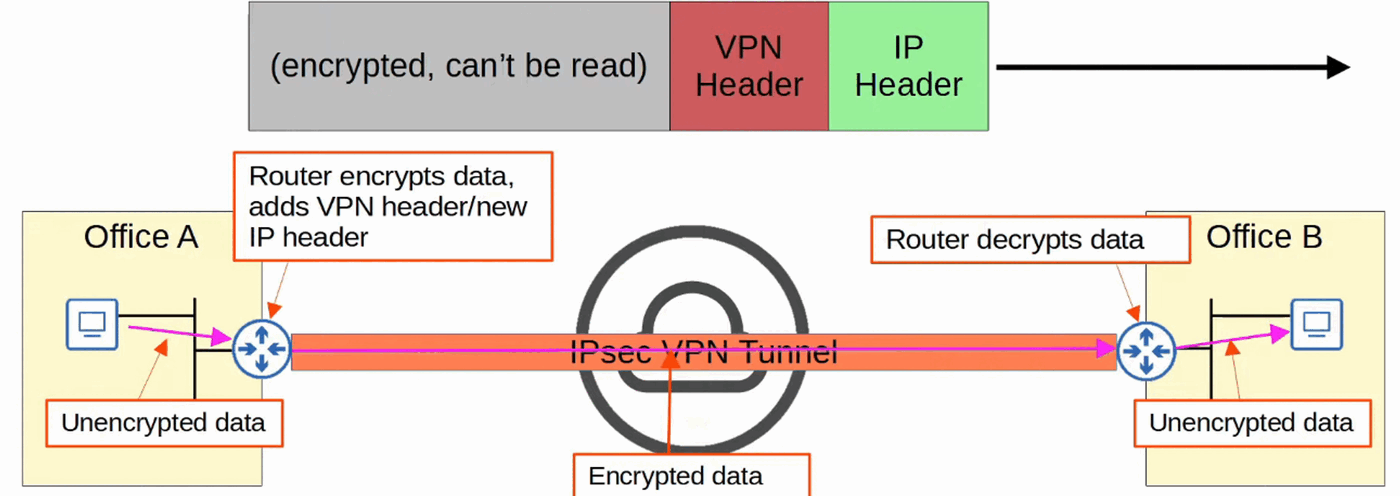
\includegraphics[keepaspectratio,alt={image}]{images/54-wan-architectures/img-014.png}}
\end{figure}

\begin{figure}
\centering
\pandocbounded{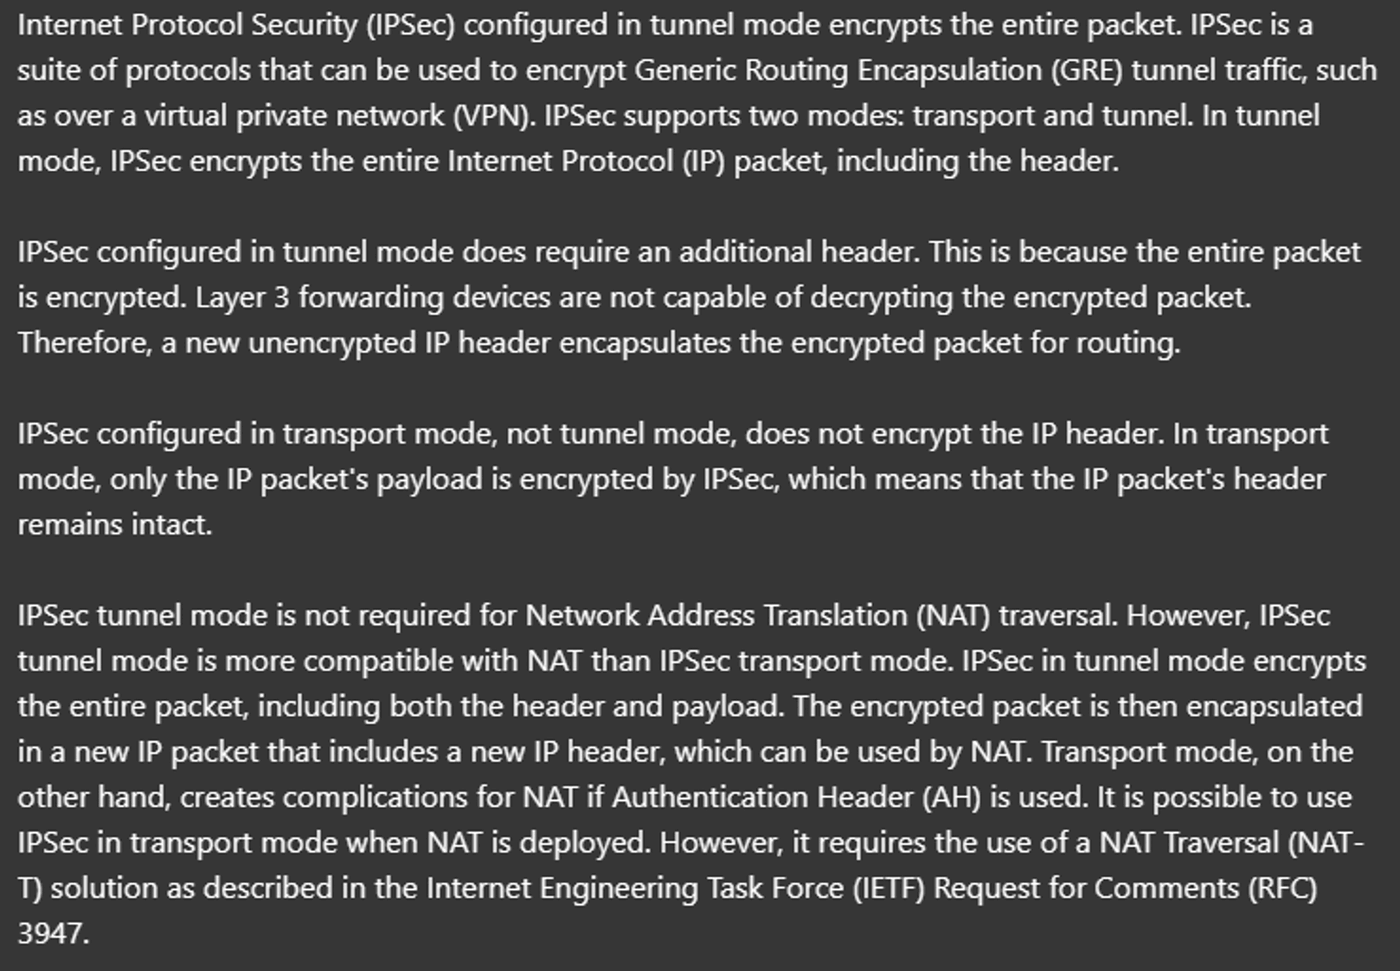
\includegraphics[keepaspectratio,alt={image}]{images/54-wan-architectures/img-015.png}}
\end{figure}

\section{Process Summary}\label{process-summary}

\begin{enumerate}
\def\labelenumi{\arabic{enumi})}
\item
  The SENDING DEVICE combines the original PACKET and SESSION KEY
  (ENCRYPTION KEY) and runs them through an ENCRYPTION FORMULA
\item
  The SENDING DEVICE encapsulates the ENCRYPTED PACKET with a VPN HEADER
  and a new IP HEADER
\item
  The SENDING DEVICE sends the NEW PACKET to the DEVICE on the other
  side of the TUNNEL
\item
  The RECEIVING DEVICE decrypts the DATA to get the original PACKET and
  then forwards the original PACKET to it's DESTINATION
\end{enumerate}

\begin{itemize}
\tightlist
\item
  In a ``SITE-TO-SITE'' VPN, a TUNNEL is formed only between TWO TUNNEL
  ENDPOINTS (for example, the TWO ROUTERS connected to the INTERNET)
\item
  All OTHER DEVICES in each site DO NOT need to create a VPN for
  themselves. They can send unencrypted DATA to their site's ROUTER,
  which will ENCRYPT it and FORWARD it in the TUNNEL as described above.
\end{itemize}

LIMITATIONS OF STANDARD IPSec

\begin{enumerate}
\def\labelenumi{\arabic{enumi})}
\tightlist
\item
  IPSec doesn't support BROADCAST or MULTICAST TRAFFIC, only UNICAST.
\end{enumerate}

\begin{itemize}
\tightlist
\item
  This means that ROUTING PROTOCOLS such as OSPF cannot be used over the
  TUNNELS because they rely on MULTICAST TRAFFIC

  \begin{itemize}
  \tightlist
  \item
    This can be SOLVED with ``GRE over IPSec''
  \end{itemize}
\end{itemize}

\begin{enumerate}
\def\labelenumi{\arabic{enumi})}
\setcounter{enumi}{1}
\tightlist
\item
  Configuring a full mesh of TUNNELS between many sites is a
  labor-intensive task
\end{enumerate}

Let's look at each of the above SOLUTIONS

GRE over IPSec

\begin{itemize}
\tightlist
\item
  GRE (GENERIC ROUTING ENCAPSULATION) creates TUNNELS like IPSec,
  however it does not ENCRYPT the original PACKET, so it is NOT SECURE
\item
  However, it has the advantage of being able to encapsulate a WIDE
  variety of a LAYER 3 PROTOCOLS as well as BROADCAST and MULTICAST
  messages
\item
  To get the FLEXIBILITY of GRE with the SECURITY of IPSec, ``GRE over
  IPSec'' can be used
\item
  The original PACKET will be ENCAPSULATED by a GRE HEADER and a new IP
  HEADER, and then the GRE PACKET will be ENCRYPTED and ENCAPSULATED
  within an IPSec VPN HEADER and a NEW IP HEADER
\end{itemize}

\begin{figure}
\centering
\pandocbounded{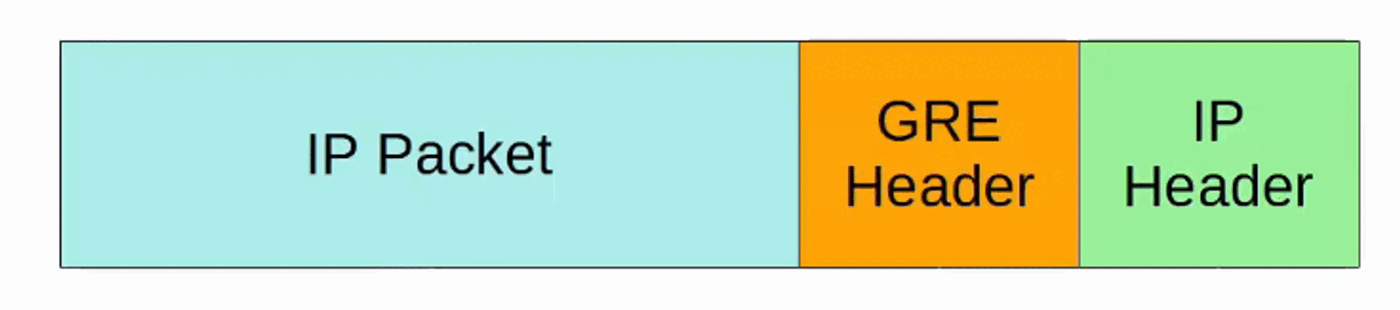
\includegraphics[keepaspectratio,alt={image}]{images/54-wan-architectures/img-016.png}}
\end{figure}

\begin{figure}
\centering
\pandocbounded{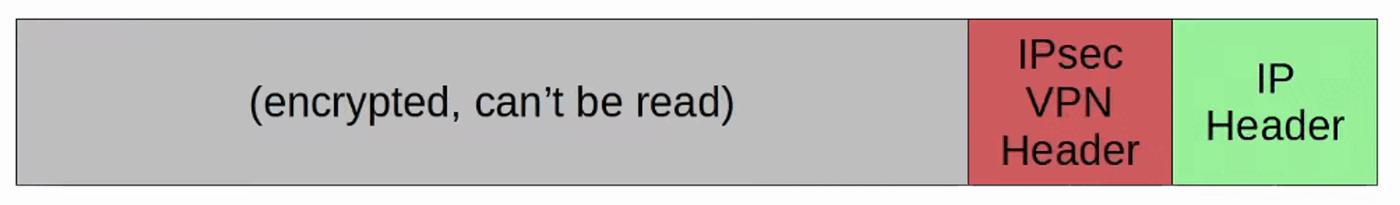
\includegraphics[keepaspectratio,alt={image}]{images/54-wan-architectures/img-017.png}}
\end{figure}

\begin{figure}
\centering
\pandocbounded{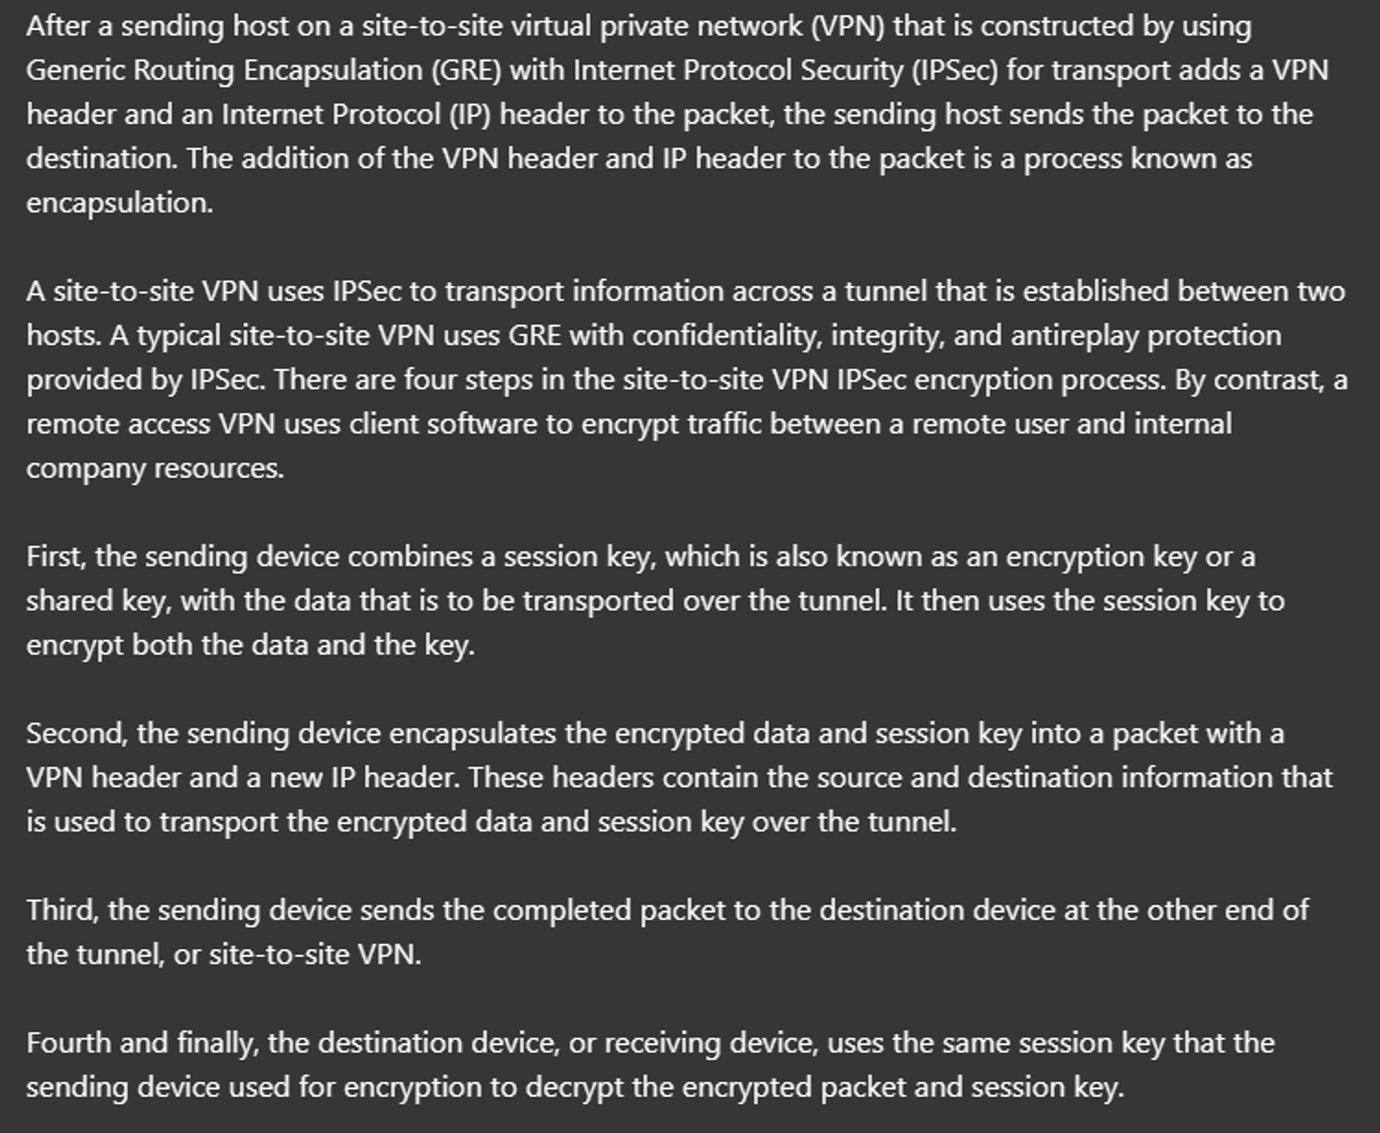
\includegraphics[keepaspectratio,alt={image}]{images/54-wan-architectures/img-018.png}}
\end{figure}

\section{DMVPN}\label{dmvpn}

\begin{itemize}
\tightlist
\item
  DMVPN (Dynamic Multipoint VPN) is a Cisco-Developed solution that
  allows ROUTERS to dynamically create a FULL MESH of IPSec TUNNELS
  without having to manually configure every SINGLE TUNNEL
\end{itemize}

\begin{enumerate}
\def\labelenumi{\arabic{enumi})}
\tightlist
\item
  CONFIGURE IPSec TUNNELS to a HUB SITE
\end{enumerate}

\begin{figure}
\centering
\pandocbounded{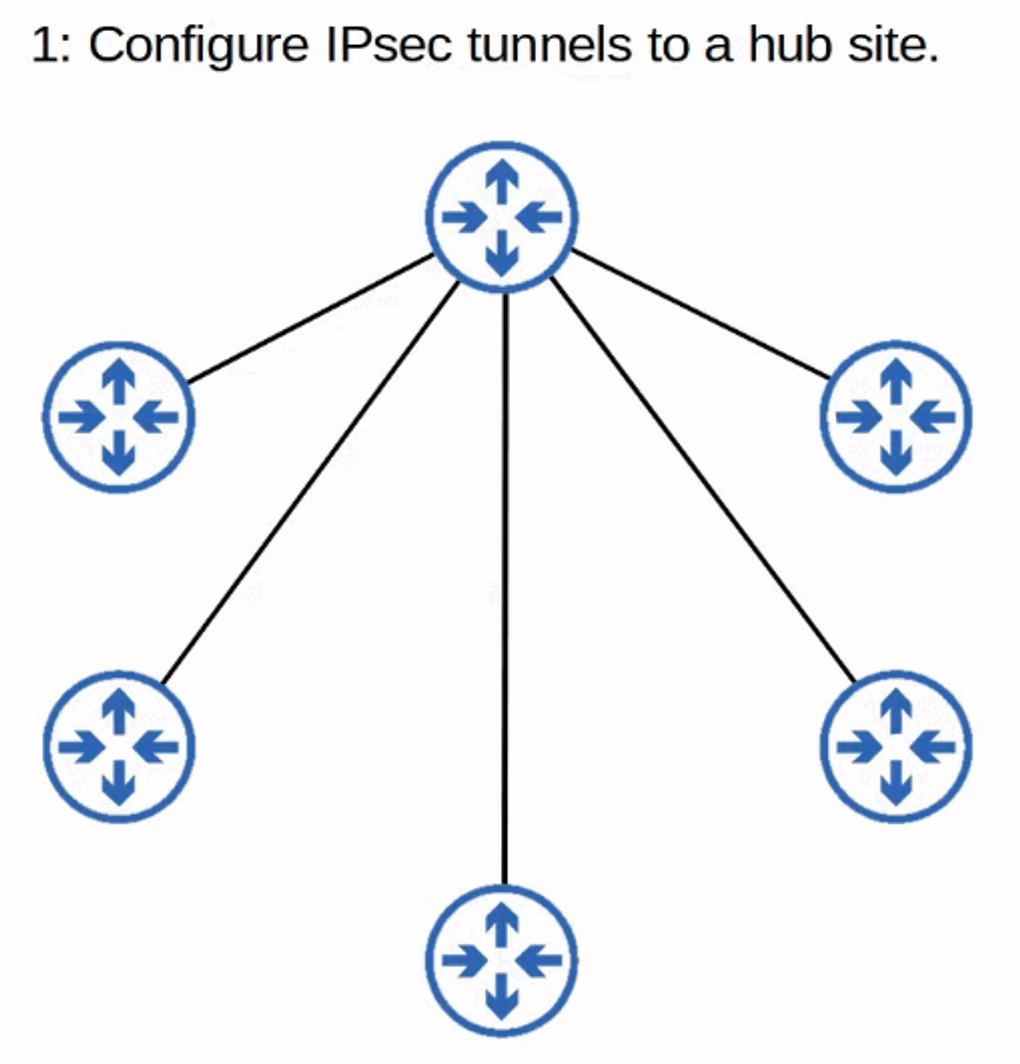
\includegraphics[keepaspectratio,alt={image}]{images/54-wan-architectures/img-019.png}}
\end{figure}

\begin{enumerate}
\def\labelenumi{\arabic{enumi})}
\setcounter{enumi}{1}
\tightlist
\item
  The HUB ROUTER gives each ROUTER information about HOW to form an
  IPSec TUNNEL with the OTHER ROUTERS
\end{enumerate}

\begin{figure}
\centering
\pandocbounded{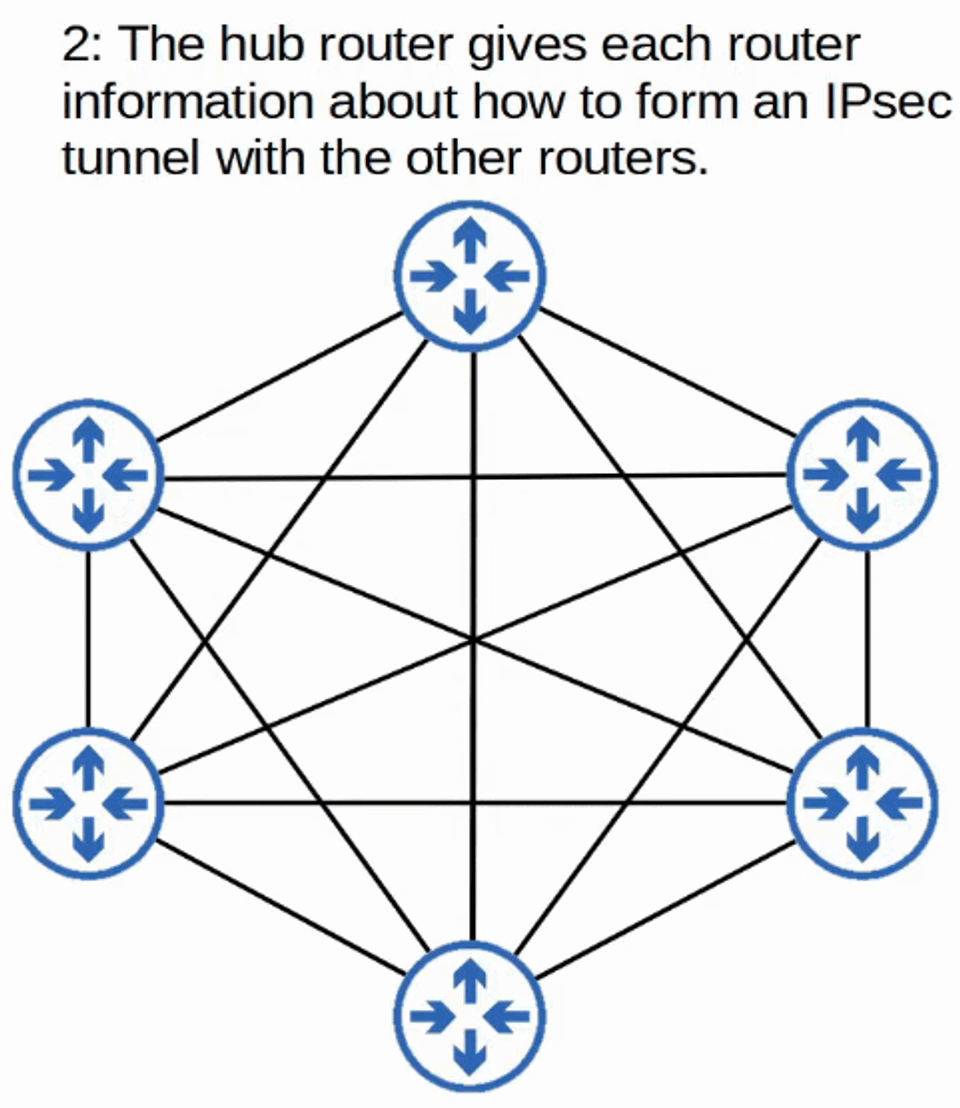
\includegraphics[keepaspectratio,alt={image}]{images/54-wan-architectures/img-020.png}}
\end{figure}

DMVPN provides the configuration simplicity of HUB-AND-SPOKE (each SPOKE
ROUTER only needs one TUNNEL configured) and the EFFICIENCY of DIRECT
SPOKE-TO-SPOKE communication (SPOKE ROUTERS can communicate directly
without TRAFFIC passing through the HUB)

REMOTE-ACCESS VPNs

\begin{itemize}
\tightlist
\item
  Whereas SITE-TO-SITE VPNs are used to make a POINT-TO-POINT connection
  between TWO SITES over the INTERNET, REMOTE-ACCESS VPNs are used to
  allow END DEVICES (PCs, Mobile Phone) to ACCESS the company's internal
  resources securely over the INTERNET
\item
  REMOTE-ACCESS VPNs typically use TLS (TRANSPORT LAYER SECURITY)

  \begin{itemize}
  \tightlist
  \item
    TLS is also what provides security for HTTPS (HTTP SECURE)
  \item
    TLS was formerly known as SSL (Secure Socket Layer) and developed by
    Netscape, but it was renamed to TLS when it was standardized by the
    IETF
  \end{itemize}
\item
  VPN client software (for example Cisco AnyConnect) is installed on END
  DEVICES (for example company-provided laptops that employees use to
  work from home)
\item
  These END DEVICES then form SECURE TUNNELS to one of the company's
  ROUTERS / FIREWALLS acting as a TLS SERVER
\item
  This allows the END USERS to securely access RESOURCES on the
  company's INTERNAL NETWORK without being directly connected to the
  company NETWORK
\end{itemize}

\begin{figure}
\centering
\pandocbounded{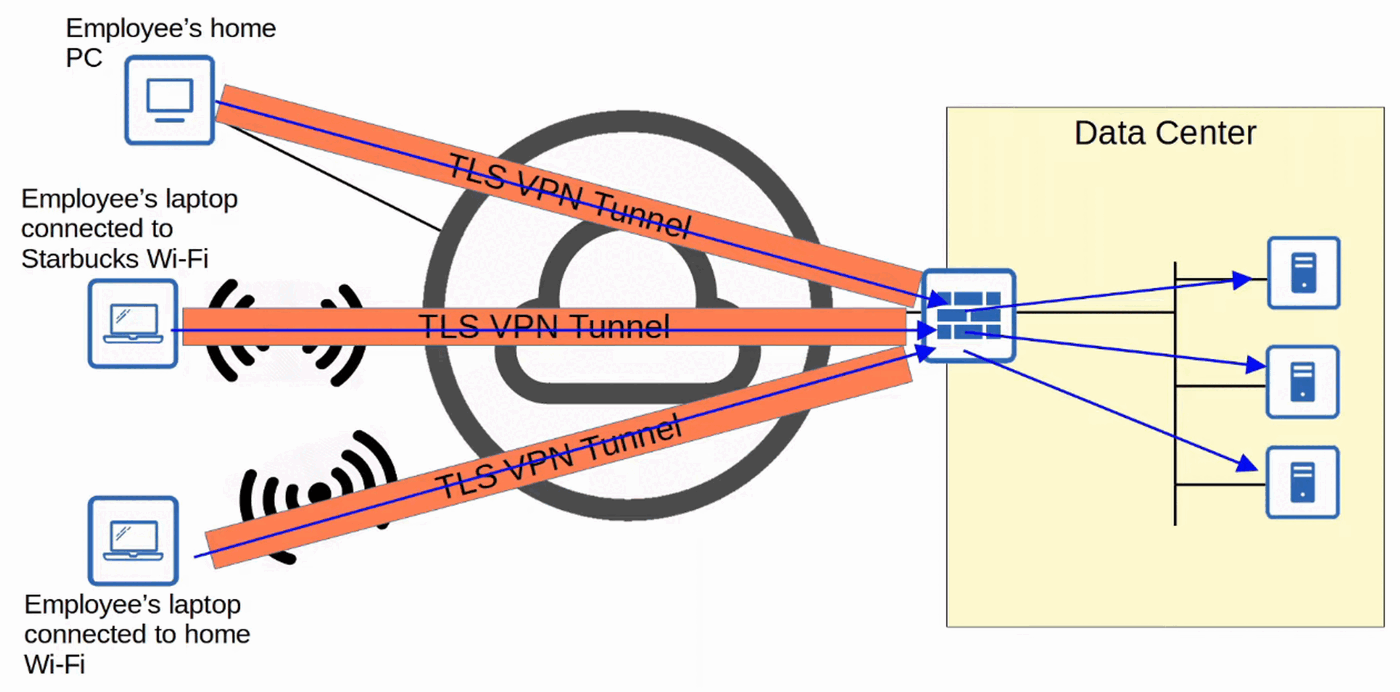
\includegraphics[keepaspectratio,alt={image}]{images/54-wan-architectures/img-021.png}}
\end{figure}

SITE-TO-SITE versus REMOTE-ACCESS VPN

\begin{itemize}
\item
  SITE-TO-SITE VPNs typically use IPSec
\item
  REMOTE-ACCESS VPNs typically use TLS
\item
  SITE-TO-SITE VPNs provide SERVICE to many DEVICES within the SITES
  they are connecting
\item
  REMOTE-ACCESS VPNs provide SERVICE to the ONE END DEVICE the VPN
  CLIENT SOFTWARE is installed on
\item
  SITE-TO-SITE VPNs are typically used to permanently connect TWO SITES
  over the INTERNET
\item
  REMOTE-ACCESS VPNs are typically used to provide ON-DEMAND ACCESS for
  END DEVICES that want to securely ACCESS company resources while
  connected to a NETWORK which is not SECURE
\end{itemize}

\section{Lab Commands}\label{lab-commands}

Create the Tunnel interface

\passthrough{\lstinline!R1(config)\#int tunnel <tunnel number>!}

This changes the mode to the Tunnel Interface

The exit interface for the tunnel

\passthrough{\lstinline!tunnel source <interface>!}

IP of the Tunnel Destination Interface

\passthrough{\lstinline!tunnel destination <destination ip address>!}

Set the IP of the Source Tunnel Interface (from step 1)

\passthrough{\lstinline!ip address <tunnel IP> <netmask>!}

Configure a Default Route to the Service Provider Network

\passthrough{\lstinline!R1(config)\#ip route 0.0.0.0 0.0.0.0 <next hop interface>!}

This will now bring the Tunnel Interface Administratively Up / Up

Now you need to set up the TUNNEL ROUTERS as OSPF Neighbors for the
Service Provider Network so they can share routes

\passthrough{\lstinline!R1(config)router ospf <ospf process ID>!}

This switches to the OSPF Router configuration mode

\passthrough{\lstinline!network <tunnel interface IP> <wildcard mask> area <area \#>!}

Since the tunnel is a single HOST, you would use 0.0.0.0 for the
Wildcard Mask

\passthrough{\lstinline!network <router gateway IP> <wildcard mask> area <area \#>!}

Since the router gateway is also a single HOST, you would use 0.0.0.0
for the Wildcard Mask

\passthrough{\lstinline!passive-interface <router gateway IP interface>!}

This removes the Router Gateway from broadcasting over OSPF
